\documentclass[11pt]{scrartcl}


\usepackage{amsmath,amsthm,amssymb}
\usepackage{hyperref}
\usepackage{mathtools}
\usepackage{enumerate}
\usepackage{graphicx}
\usepackage{mathpazo}
\usepackage{lmodern}
\usepackage{parskip}

\theoremstyle{plain} 
\newtheorem{theorem}{Theorem}
\newtheorem{lemma}[theorem]{Lemma}
\newtheorem{algorithm}{Algorithm}
\DeclarePairedDelimiter\ceil{\lceil}{\rceil}
\DeclarePairedDelimiter\floor{\lfloor}{\rfloor}


\theoremstyle{definition}
\newtheorem*{definition}{Definition} 
\theoremstyle{remark}
\newtheorem{remark}{Remark}


\usepackage[margin=1in]{geometry}

\usepackage{fancyhdr}
\pagestyle{fancy}
\lhead{15-418 Writeup}
\rhead{Jacob Imola (jimola), Sidhanth Mohanty (smohant1)} 
\cfoot{\thepage}

\DeclareMathOperator{\Tr}{\mathsf{Tr}}

\newcommand{\half}{\frac{1}{2}}
\newcommand{\cbrt}[1]{\sqrt[3]{#1}}
\newcommand{\Prob}{\textbf{Pr}}
\newcommand{\eps}{\varepsilon}
\newcommand{\E}{\textbf{E}}
\newcommand{\Ind}{\boldsymbol{1}}
\newcommand{\Ener}{\mathcal{E}}
\newcommand{\Var}{\textbf{Var}}
\newcommand{\rank}{\mathsf{rank}}
\newcommand{\frontier}{\texttt{frontier}}
\newcommand{\info}{\texttt{info}}
\newcommand{\waiters}{\texttt{waiters}}
\begin{document}

\title{15-418 Project Proposal: Parallel Low Diameter Decompositions in Graphs}
\author{\textsf{Jacob Imola (jimola), Sidhanth Mohanty (smohant1)}}
\date{\textsf{\today}}
\maketitle

\section{Summary}
We implemented an algorithm from a paper of Gary Miller, Richard Peng and Shen Xu \cite{miller2013parallel}
to perform a low diameter decomposition in graphs in parallel using \texttt{C++} and \texttt{OpenMP}.
Depending on the structure of the graph, we achieved somewhere between a $2$-$3\times$ when using all
the cores on a single machine in \texttt{latedays} compared to the single threaded implementation of
this algorithm. We also implemented a work efficient simple sequential algorithm, and unfortunately,
on some sparse graphs, the sequential algorithm is more efficient.

\section{Background}
A low diameter decomposition of a graph is a partition of the vertices of the graph into clusters such
that the distance between any two vertices inside a single cluster is small and the number of edges
between any two clusters is small compared to the total number of internal edges. Formally, an $(\alpha,
\beta)$ LDD of the graph is a decomposition of $V$ into disjoint $V_1,V_2,\ldots,V_t$ such that for
any $v_1,v_2\in V_i$, $d(v_1,v_2)\leq\alpha$ and the number of edges leaving $V_i$ is at least a
$\beta$ fraction of the number of internal edges in $V_i$.

The baseline sequential algorithm to find a $(\frac{\log n}{\beta},\beta)$-LDD works in the following way:
pick a vertex and start a BFS and stop when the fraction of edges leaving the current component is less
than $\beta(\text{number of internal edges})$. Put all the visited vertices in a cluster and recurse on the
remaining graph.

The reason this algorithm is not nicely parallelizable is that picking clusters is an inherently sequential process.
Miller, Peng, and Xu \cite{miller2013parallel} propose an algorithm (MPX) to bypass this limitation, which we describe below:

\begin{enumerate}

\item Assign a value $\delta_u\sim\text{Exp}(\beta)$ to each vertex $u$ (a parallel step). This value is the amount of ``head start'' that each vertex gets.

\item Compute $\delta_{\text{max}} = \max\{\delta_u|u\in V\}$, and set the start times of vertex $u$ as $\delta_{\text{max}}-\delta_u$.

\item Do a single BFS, where each vertex in the frontier belongs to a cluster and set any neighbors in the next frontier to the same cluster. Each round of BFS takes 1 second, and a vertex $v$ with start time $S$ joins the frontier at round $\lfloor S \rfloor$ with its own cluster if it hasn't already been visited. We store $S-\lfloor S \rfloor$ as a tiebreaker; if a vertex $u$ in the next frontier hit by multiple vertices in the current frontier, $u$ belongs to the cluster of the vertex with the smallest tiebreaker.

\end{enumerate}
It is not hard to see that a vertex will belong to the cluster of the vertex that has the minimum distance plus start time. Steps 1 and 2 are extremely parallelizable. Step 3 involves a single BFS, so its parallelization depends on the topology of the graph. For each vertex, we store the cluster it belongs to, its minimum tiebreaker, and its start time in an array called $\info$. Each frontier is represented as an array called $\frontier$. Finally, we have an array called $\waiters$ that keeps track of vertices that haven't entered the BFS yet. The parallelism comes from the fact that we can initialize $\info$ and go through $\frontier$ and $\waiters$ in parallel. Note that on a sparse graph with high diameter, there is not much parallelism.


\section{The Approach}
We used \texttt{C++} with \texttt{OpenMP} and optimized our code on the \texttt{latedays} machine.

\begin{itemize}
\item In the first step of initializing $\info$, we,
we run a \texttt{\#pragma omp parallel for} loop to
have multiple threads assign values to different vertices
at the same time. We also needed an array of locks, $\texttt{locks}$, to make sure that only one thread can update tiebreakers and clusters in $\info$ at once.

\item Although the max can be computed using a reduce, we do
it sequentially since the advantage of reduce is noticable
only in a large number of cores.

\item We represent $\frontier$ using a vector. To construct a new frontier, we ran through $\frontier$ in parallel (using dynamic scheduling), and each thread sees if a neighbor hasn't been visited or has a lower tiebreaker than what is in $\info$. If this is the case, it updates $\info$ to reflect the lower tiebreaker (using locks), adds the vertex to its personal vector of vertices, $\texttt{new\_frontier}_t$ for each thread $t$. Then, a thread sequentially goes through $\texttt{new\_frontier}_t$ for every $t$, updates $\info$, and puts every unique vertex into a single vector for the next frontier. \par
\item We realized that we could represent $\waiters$ distributed over each thread, and each thread's slice of $\waiters$ will be more-or-less the same size due to the random wait times. This avoids the needs for locks and provides good parallelism.

\end{itemize}

We spent a lot of time deciding how to represent $\frontier$ and $\waiters$. We were tempted to let both be arrays be 0/1 indicator arrays, but we didn't want $O(n)$ work to occur on each iteration, even if this work occurred in parallel. We then tried representing $\frontier$ as a vector and build $\texttt{new\_frontier}$ with a single, coarse lock on it, but there was too much contention for this lock, especially if the vector is resized. We decided that if we could reduce the granularity of locking, and then do a sequential $O(|F|)$ pass of the frontier (where $|F|$ is the size of the new frontier) at the end, it would be a simple solution that would beat the overhead of more complicated data structures and would only result in $O(n)$ sequential work at the end of the algorithm.

\par We accomplished this by giving a lock to each vertex, and having $\texttt{new\_frontier}$ be distributed. The contention for these locks is relatively low but grows as the degree of the vertex grows. A vertex is added to $\texttt{new\_frontier}_t$ only if it is unvisited and beats the current tiebreaker. There could be repeats in $\texttt{new\_frontier}$, but since the tiebreakers are random, the expected number of vertices will be $O(|F|\log d)$, where $d$ is the maximum degree of the graph. This results in $O(|F|\log n)$ sequential work to combine the vertices, but in most graphs, it will be very close to $O(|F|)$.

\par
We could have done the same thing for $\waiters$, but we realized there is a lock-free solution, which means even less overhead. We simply distributed $\waiters$ over all available threads, again taking advantage of the fact that the wait times are random. This means that the workload distribution will be good in expectation. The total work in this step is $O(\frac{n}{\beta})$ which they prove in the paper. We could have sorted $\waiters$ at an $O(n \log n)$ upfront cost and only have had $O(n)$ work throughout the whole algorithm, but we decided against this because we thought the first method was fast enough, and was simpler.

\begin{figure}
\begin{minipage}[c]{0.5\textwidth}
\begin{center}
	
\includegraphics[scale=0.2]{grid_seq.png}
\end{center}
\end{minipage}
\begin{minipage}[c]{0.5\textwidth}
\begin{center}
	
\includegraphics[scale=0.2]{grid_mpx.png}
\end{center}
\end{minipage}
\caption{Clusters produced by sequential (left) and MPX (right) on 1000x1000 grid for $\beta=0.05$}
\label{fig:1}
\end{figure}

\section{Results}
To measure the performance of our implementation, we tested it on three types of large graphs with three different values of $\beta$ with 1, 2, 4, 8, and 16 threads given to OpenMP. We compared this to the runtime of the single-threaded sequential algorithm. We measured the runtime in seconds using \texttt{CycleTimer} as we have used in class. The three graphs that we tested are described below:
\begin{itemize}
\item Graph A: A power-law graph, meaning that the degrees are distributed according to a power-law, generated randomly from Stanford's SNAP library, with 500,000 vertices and average degree 10. This graph represents what a typical social network or real-world graph may look like.
\item Graph B: A 1000x1000 grid graph. This graph has poor parallelization potential, but it's a good edge-case and it's easy to plot the clusters that are produced (Figure \ref{fig:1}).
\item Graph C: 500 cliques of size 300 that are connected to each other via a tree. This graph has very clear clusters, large average degree, and a very low diameter, so the parallelism opportunities are large.
\end{itemize}

\begin{figure}
\vspace*{-3cm}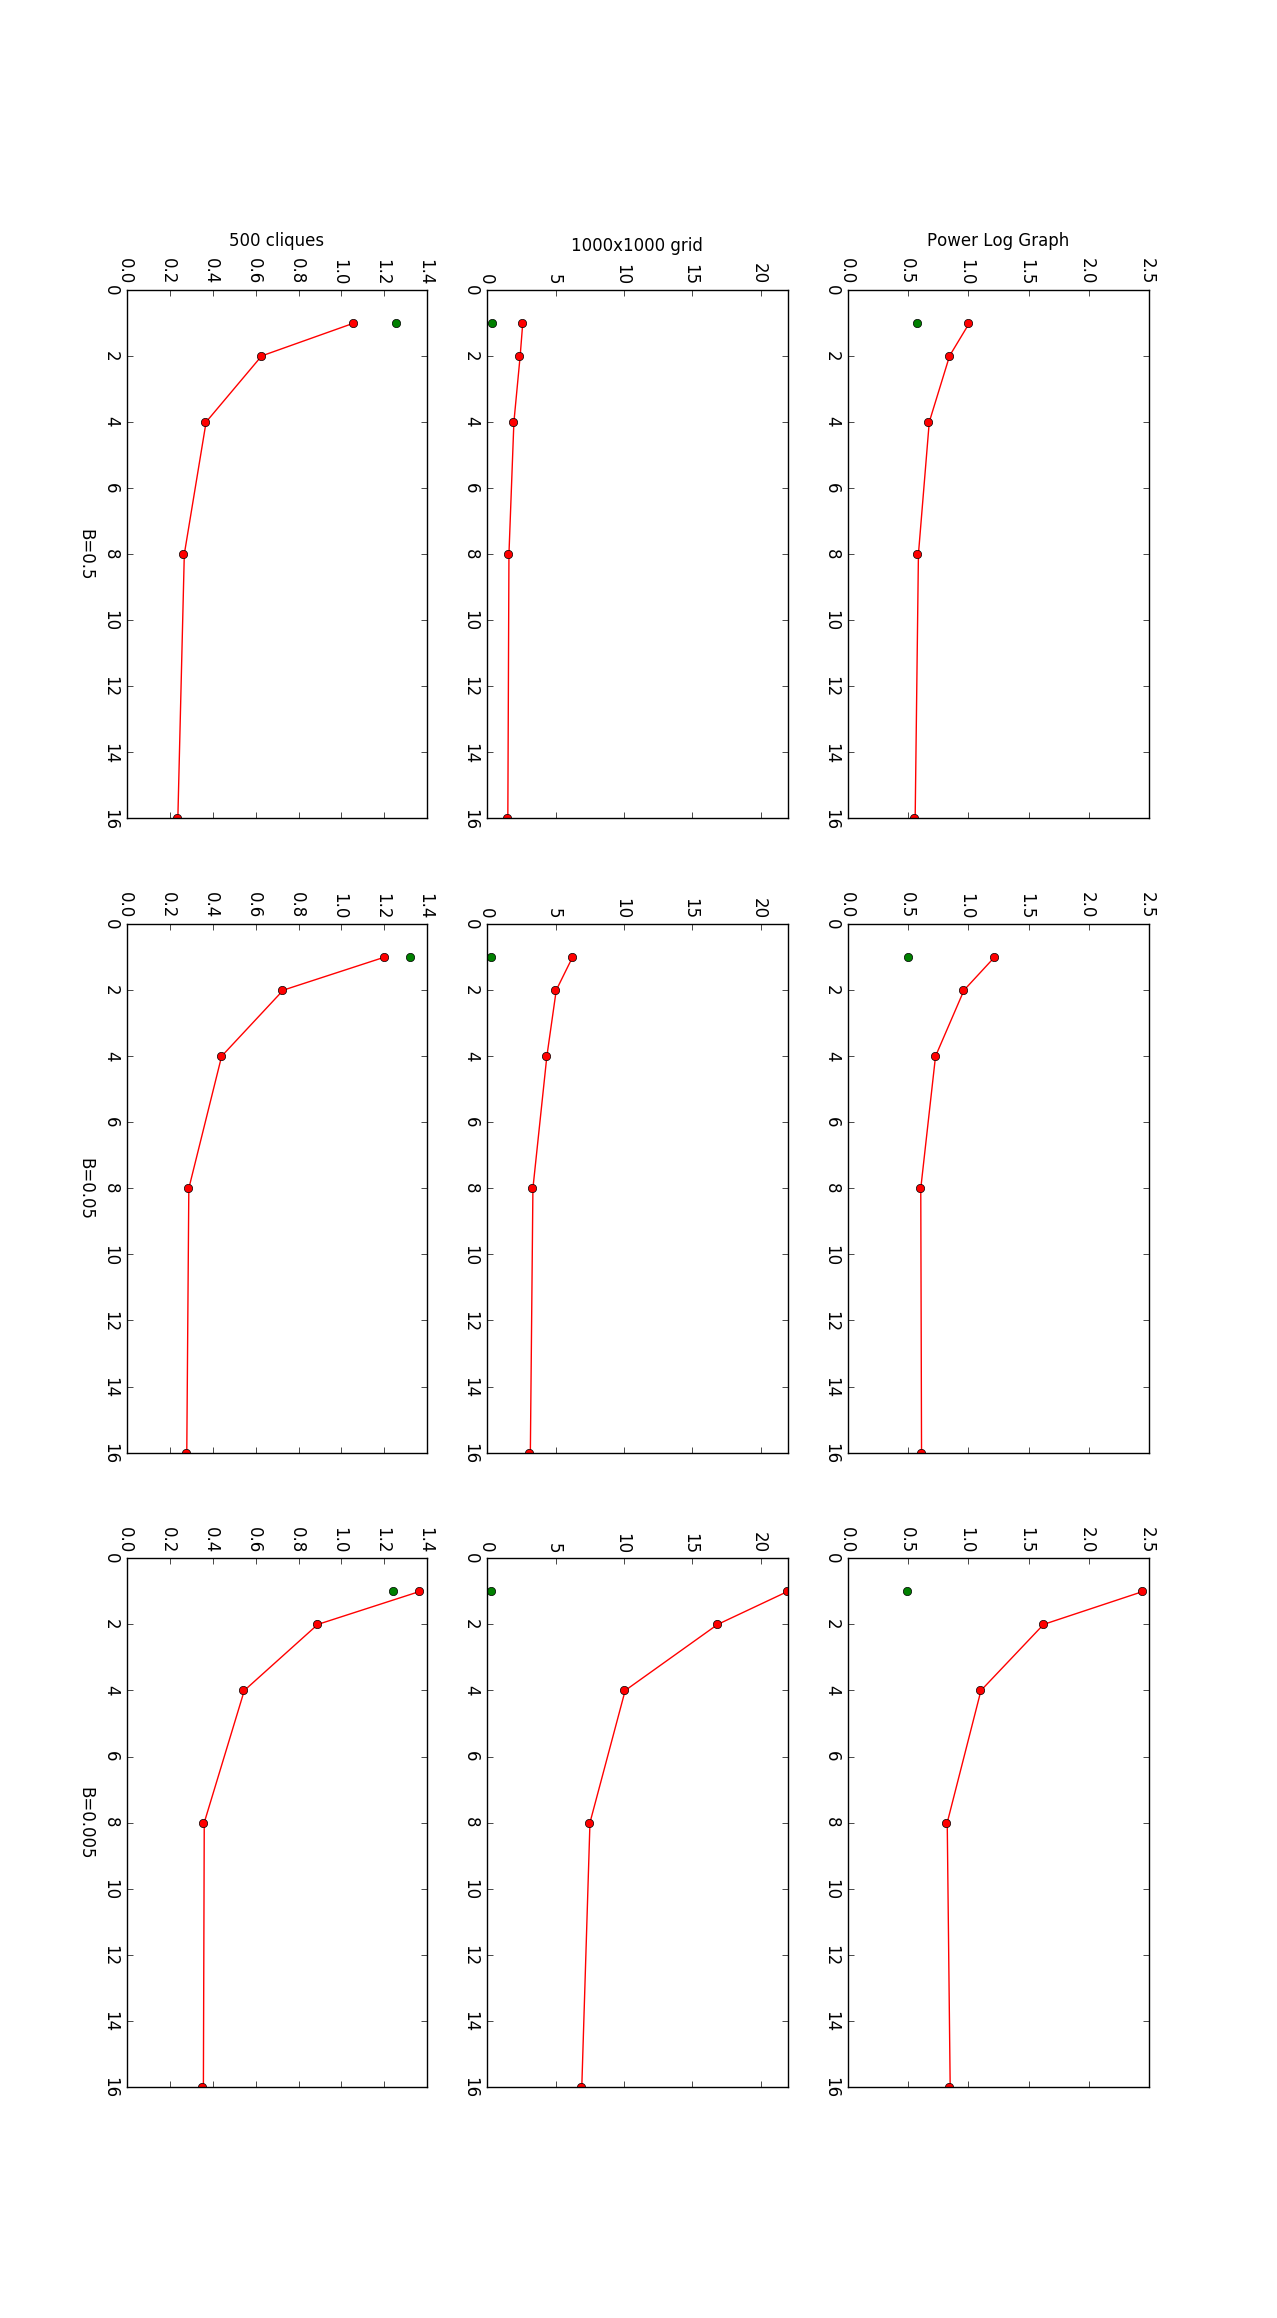
\includegraphics[width=\textwidth]{Speedup_plots.png}\vspace{-3cm}
\caption{Speedup plots for 3 different graphs and 3 different values of $\beta$.}
\label{fig:2}
\end{figure}

\begin{figure}
\begin{center}
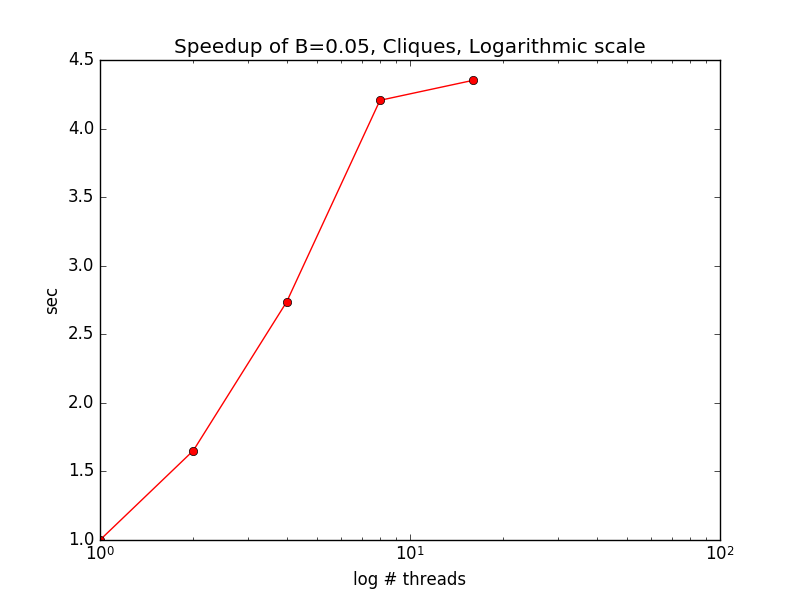
\includegraphics[scale=0.5]{Log_scale.png}
\end{center}
\caption{Cliques graph with $\beta=0.05$ with x-axis on a log scale; there is a near-linear speedup until 16 threads}
\label{fig:3}
\end{figure}
The speedup plots (Figure \ref{fig:2}) reveal a number of interesting facts about the two implementations. Notice that, in most cases, the 1-processor runtime of MPX is greater than the sequential algorithm. This represents the overhead of using locks and randomness, as well as having $\waiters$. However, we do see that MPX is very parallelizable, and the only sequential part is the number of BFS steps we must perform. Graph B showed the lowest speedup because it has a high diameter, but Graph C has very close to perfect speedup until 16 threads (Figure \ref{fig:3}), where it is plotted with a logarithmic scale. The less good speedup for 16 threads can be explained because \texttt{latedays} has only 12 cores. \par

The amount of time spent iterating through $\waiters$ is proportional to $\frac{1}{\beta}$. This explains why, as $\beta$ decreases, the runtimes increase drastically.  This problem is compounded in graph B, because vertices are not visited for a long time and they remain in $\waiters$. When $\beta=0.005$, the sequential algorithm is over 100x faster than MPX with one thread. This highlights a drawback with our implementation of MPX, as its runtime depends on $\frac{1}{\beta}$. Sorting $\waiters$ beforehand would fix this problem, but for high values of $\beta$, sorting would be more work. \par

Our algorithm truly shines on high values of $\beta$ on graphs with low diamter. In fact, graph C for $\beta=0.5$ and $\beta=0.05$ are actually faster than the sequential algorithm for 1 thread. This is because the sequential algorithm has overhead where it must somehow count the number of edges going out of its current frontier, and if it decides to stop the BFS there, then it must roll back its changes which is poor for cache locality. MPX circumvents this problem because once a vertex is visited, it's final.

\par
The most realistic graph, graph A, has a mixed result for MPX. When $\beta = 0.5$, MPX does manage to beat the sequential algorithm with 8 or more cores. For the smaller values of $\beta$, the overhead of $\waiters$ is too much, and it fails to beat the sequential.
 

\section{List of work by each student}
\begin{itemize}
\item \textbf{Jacob:} Implemented the Miller-Peng-Xu
algorithm and parallelized it in OpenMP, also optimized
and improved the sequential baseline written by Sidhanth.
Also wrote the setup code in \texttt{main.cpp}.

\item \textbf{Sidhanth:} Wrote the sequential baseline and
performed some optimizations on the MPX algorithm.

\end{itemize}

\bibliographystyle{alpha}
\bibliography{project_proposal}

\end{document}
